

% ======== 正文 ==============================

\section{引言}
此文档面向测试中心性能和可靠性测试实验室相关人员,主要目的是如何完成将测试数据利用工具自动填写到准备好的测试报告模版中。如果有任何问题,请联系:q30china@gmail.com. 

%\section{正文}

\vspace*{0.2cm}
\begin{center}
    \Huge 测试报告数据自动映射工具说明
\end{center}
\vspace{0cm}

\section{安装}

本工具为python编写,可跨平台使用。为了让实验室人员方便使用,本文的例子和截图全部针对Windows平台。MacOS和Linux不在此说明。

\subsection{安装运行环境}

\begin{lstlisting}
# 打开命令提示符(CMD)或PowerShell
# 导航到你的项目目录:
cd d:\autotable

# 双击安装python3.13
python-3.13.0-amd64.exe

# 创建python虚拟环境,在当前目录下生成一个.venv的文件
python -m venv .venv

# 进入虚拟环境
d:\autotable\.venv\Scripts\activate.bat

# 出现如下提示符,证明已经进入虚拟环境
(.venv) d:\autotable\.venv\Scripts>

# 在项目目录安装项目所需要的包 (大约等待)
d:\autotable\pip install -r requirements

\end{lstlisting}

\subsection{初始化检查}
这是项目当前的目录结构:
\begin{figure}[H]
    \begin{center}
        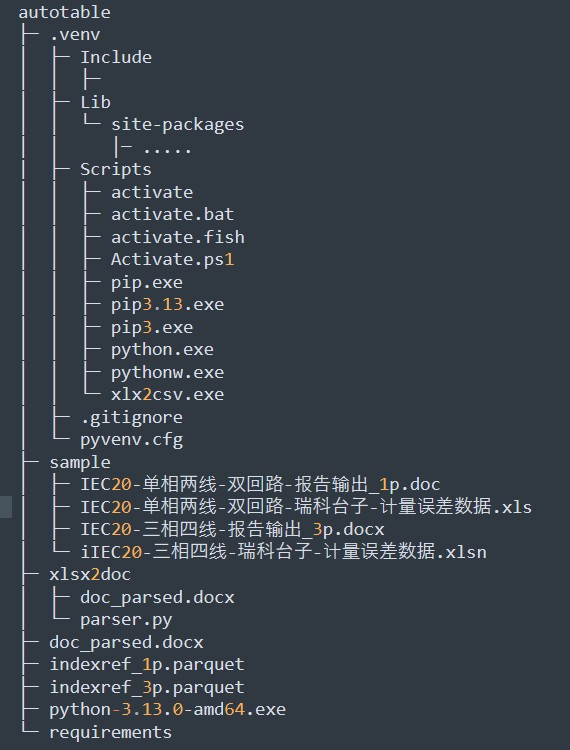
\includegraphics[width=.5\linewidth]{res/dir.jpg}\\
        \caption{autotable directory structure }\label{dir}
    \end{center}
\end{figure}

确保python主程序中的目录和实际目录一致,包括单三相表的报告模版文件名称和数据格式都要一致。

\begin{minted}[frame=single,framesep=1mm,breaklines=true]{python}
def main() -> None:
    ps = Parser('D:/autotable/sample/IEC20-三相四线-报告输出_3p.docx')
    ps.parse_3p_excel_table('D:/autotable/sample/IEC20-
    三相四线-瑞科台子-计量误差数据.xls')
    ps.map_excel_to_docx_table('D:/autotable/indexref_3p.parquet')
    
    # ps = Parser('D:/autotable/sample/IEC20-单相两线-双回路-报告输出_1p.docx')
    # ps.parse_1p_excel_table('D:/autotable/sample/IEC20-单相两线-双回路-瑞科台子-计量误差数据.xls')
    # ps.map_excel_to_docx_table('D:/autotable/indexref_1p.parquet')
\end{minted}

\section{运行}

在虚拟环境中运行主程序,默认完成三相四线电表的数据自动映射
\begin{lstlisting}
# 在项目目录里运行命令
(.venv) d:\autotable>python  ./xlsx2doc/parser.py
\end{lstlisting}

执行速度很快,以下为输出结果,输出测试报告带数据映射

\begin{figure}[H]
    \begin{center}
        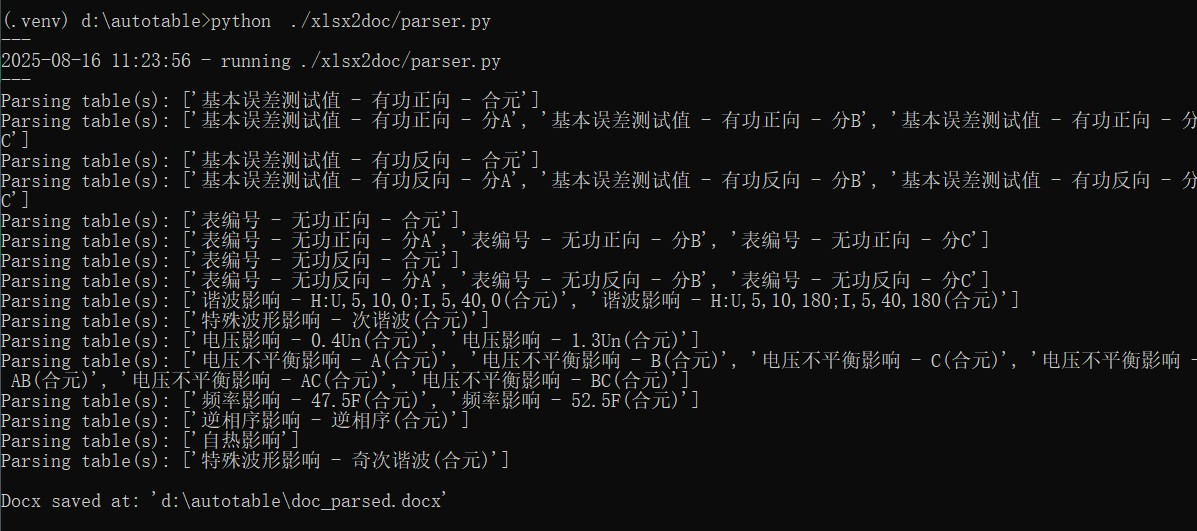
\includegraphics[width=.95\linewidth]{res/results.jpg}\\
        \caption{Results}\label{resultes}
    \end{center}
\end{figure}

